
\documentclass[a4paper,12pt]{article} \usepackage{graphicx}
\usepackage{epstopdf} %\usepackage{gensymb} \usepackage{longtable}
\usepackage{graphicx}
\usepackage{listings}
\usepackage{caption}
\usepackage{subcaption}
\usepackage{morefloats}
\lstset{
        language=verilog,
        basicstyle=\footnotesize,
        breaklines=true
}

%% Definitioner för LIPS-dokument

\usepackage[english,swedish]{babel}
\usepackage[utf8]{inputenc}
\usepackage[T1]{fontenc}
\usepackage{times}
\usepackage{ifthen}

\usepackage[margin=25mm]{geometry}

\usepackage{fancyhdr}
\pagestyle{fancy}
\lhead{}
\chead{\textbf{\LIPSprojekttitel}}
\rhead{\textbf{\textsl{LiTH}}\\\textbf{\LIPSdatum}}
\lfoot{\textbf{\LIPSkursnamn}\\\textbf{\LIPSdokumentansvarig}}
\cfoot{\textbf{\LIPSprojektgrupp}\\\textbf{\LIPSgruppepost}}
\rfoot{\textbf{\textsc{Lip}s}\\\textbf{Sida~\thepage}}

\setlength{\parindent}{0pt}
\setlength{\parskip}{1ex plus 0.5ex minus 0.2ex}


\newcommand{\twodigit}[1]{\ifthenelse{#1<10}{0}{}{#1}}
\newcommand{\dagensdatum}{\number\year-\twodigit{\number\month}-\twodigit{\number\day}}

%% ------------------------------------------
% NYBILD
% Skapar centrerad bild med caption
%   
% #1: Filens url relativt '/bilder/'
% #2:  Caption
% #3: Label
% #4: Skalning
%% ------------------------------------------
\newcommand{\nyBild}[4] 
{\begin{figure}[H]
  \centering
 \includegraphics[angle=0,scale=#4]{bilder/#1}
  \caption{#2}
  \label{fig:#3}
\end{figure}}



%%  Redefinitions of commands containing @
\makeatletter
\makeatother

\newcommand{\LIPStitelsida}{%
{\ }\vspace{45mm}
\begin{center}
  \textbf{\Huge \LIPSdokumenttyp}
\end{center}
\begin{center}
  {\Large Editor: \LIPSredaktor}
\end{center}
\begin{center}
  {\Large \textbf{Version \LIPSversion}}
\end{center}
\vfill
\begin{center}
  {\large Status}\\[1.5ex]
  \begin{tabular}{|*{3}{p{40mm}|}}
    \hline
    Reviewed & \LIPSgranskare & \LIPSgranskatdatum \\
    \hline
    Approved & \LIPSgodkannare & \LIPSgodkantdatum \\
    \hline
  \end{tabular}
\end{center}
\newpage
}


\newenvironment{LIPSprojektidentitet}{%
{\ }\vspace{45mm}
\begin{center}
  {\Large PROJECT IDENTITY}\\[0.5ex]
  {\small
  \LIPSartaltermin, \LIPSprojektgrupp\\
  Linköpings Tekniska Högskola, ISY
  }
\end{center}
\begin{center}
  {\small Group member}\\
%  \begin{tabular}{|p{30mm}|p{40mm}|p{35mm}|p{45mm}|}
  \begin{tabular}{|l|p{45mm}|p{25mm}|l|}
    \hline
    \textbf{Name} & \textbf{Responsibility} & \textbf{Phone} & \textbf{E-mail} \\
    \hline
}%
{%
    \hline
  \end{tabular}
\end{center}
\begin{center}
  {\small
    %\textbf{E-postlista för hela gruppen}: \LIPSgruppepost\\
    %\textbf{Hemsida}: \LIPSgrupphemsida\\[1ex]
    \textbf{Customer}: \LIPSkund\\
    \textbf{Customer Contact}: \LIPSkundkontakt\\
    \textbf{Course Leader}: \LIPSkursansvarig\\
    \textbf{Tutor}: \LIPShandledare\\
  }
\end{center}
\newpage
}
\newcommand{\LIPSgruppmedlem}[4]{\hline {#1} & {#2} & {#3} & {#4} \\}



\newenvironment{LIPSdokumenthistorik}{%
\begin{center}
  Document history\\[1ex]
  \begin{small}
    \begin{tabular}{|l|l|p{60mm}|l|l|}
      \hline
      \textbf{Version} & \textbf{Date} & \textbf{Changes} & \textbf{Edited by} & \textbf{Reviewed} \\
      }%
    {%
      \hline
    \end{tabular}
  \end{small}
\end{center}
}
\newcommand{\LIPSversionsinfo}[5]{\hline {#1} & {#2} & {#3} & {#4} & {#5} \\}

\newcounter{LIPSkravnummer}
\newcounter{LIPSunderkravnummer}[LIPSkravnummer]

\newenvironment{LIPSkravlista}{%
  \begin{tabular}{|p{25mm}|p{25mm}|p{85mm}|p{5mm}|}
    }%
  {%
    \hline
  \end{tabular}
}

\newenvironment{LIPSleveranslista}{%
  \begin{tabular}{|p{25mm}|p{20mm}|p{65mm}|p{25mm}|p{5mm}|}
    }%
  {%
    \hline
  \end{tabular}
}


\newcommand{\LIPSkrav}[3]
{\hline
\stepcounter{LIPSkravnummer}\textbf{Krav nr \arabic{LIPSkravnummer}} &
\textbf{{#1}} & 
{#2} & 
\textbf{{#3}} 
\\}

\newcommand{\LIPSleverans}[4]
{\hline
        \textbf{{#1}} & 
        {#2} & 
        {#3} & 
        \textbf {{#4}} 
\\}

\newcommand{\LIPSunderkrav}[3]{\hline\stepcounter{LIPSunderkravnummer}\textbf{Requirement nr \arabic{LIPSkravnummer}\Alph{LIPSunderkravnummer}} & \textbf{{#1}} & {#2} & \textbf{{#3}} \\}





%%% Local Variables: 
%%% mode: latex
%%% TeX-master: "kravspec_mall"
%%% End: 


\newcommand{\degree}{\ensuremath{^\circ}}
\newcommand{\LIPSartaltermin}{2013/VT}
\newcommand{\LIPSkursnamn}{TSEK06}
\newcommand{\LIPSprojekttitel}{DLL Based Frequency Multiplier}

\newcommand{\LIPSprojektgrupp}{Group 7}

\newcommand{\LIPSgruppepost}{}
\newcommand{\LIPSgrupphemsida}{} 
\newcommand{\LIPSdokumentansvarig}{Gustav Svensk}

\newcommand{\LIPSkund}{ISY, Linköpings universitet, 581\,83 Linköping}

\newcommand{\LIPSkundkontakt}{Amin Ojani}
\newcommand{\LIPSkursansvarig}{Atila Alvandpour}
\newcommand{\LIPShandledare}{Amin Ojani}

\newcommand{\LIPSdokumenttyp}{Layout Design} 
\newcommand{\LIPSredaktor}{Nora Björklund} 
\newcommand{\LIPSversion}{1.0} 
\newcommand{\LIPSdatum}{\dagensdatum}

\newcommand{\LIPSgranskare}{} 
\newcommand{\LIPSgranskatdatum}{}
\newcommand{\LIPSgodkannare}{} 
\newcommand{\LIPSgodkantdatum}{}

\begin{document}
\LIPStitelsida

%% Argument till \LIPSgruppmedlem: namn, roll i gruppen, telefonnummer, epost
\selectlanguage{swedish}
\begin{LIPSprojektidentitet}
 
\LIPSgruppmedlem{Nora Björklund}{Project leader}{076 7756
789}{norbj648@student.liu.se}
\LIPSgruppmedlem{\LIPSdokumentansvarig}{Documentation}{073
6208776}{grulfen3@gmail.com} 
\LIPSgruppmedlem{Christopher Hallberg}{}{0739845945}{chrha007@student.liu.se} 
\LIPSgruppmedlem{Gustaf Bengtz}{}{0707367307}{gbengtz@gmail.com} 
\LIPSgruppmedlem{Johan Berneland}{}{0704988329}{johbe915@student.liu.se}
\end{LIPSprojektidentitet}

\selectlanguage{english}

\tableofcontents{} 
\newpage %% Argument till \LIPSversionsinfo: versionsnummer, datum, Ändringar,
         %  utfört av,granskat av
\addcontentsline{toc}{section}{Document history}
\begin{LIPSdokumenthistorik} 
        \LIPSversionsinfo{0.1}{}{First draft.}{}{}
\end{LIPSdokumenthistorik} 
\newpage

\section{Time Report}
% Bifogas

\section{Project Desciption}
% Kort beskrivning med motivering och mål.
% Blocknivå beskrivning liknande från tidigare rapporter

The complete system

\begin{figure}[h]
\centering
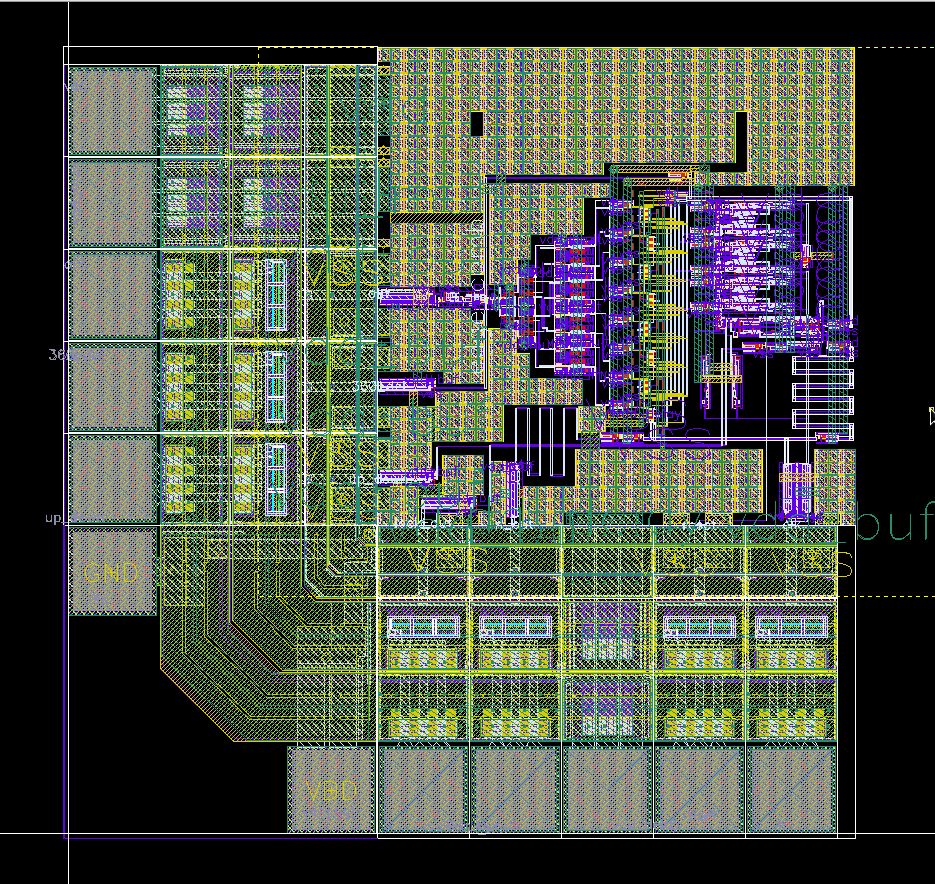
\includegraphics[width=\textwidth]{../Bilder/Layout/complete_system_pad.png}
\caption{Complete system}
\label{fig:complete_system_pad}
\end{figure}

\subsection{Phase Detector}
The Phase Detector (PD) is used check whether the 360\degree delayed
signal has got a rising edge before or after the system clock. If the
360\degree delayed clock rises before the system clock, the output
from the PD is 0, and if it rises after the system clock the output is 1.
This is used to tell the counter whether it should count up or down. 

The final layout of the PD can be seen in \ref{fig:pd_final} in appendix \ref{sec:Layout}.
\subsection{Counter}
The purpose of the counter is to generate the control signals for the delay line.
The counter is a six bit up/down counter with synchronous reset and both
inverted and non-inverted outputs. It is controlled by two signals, an enable
signal which is generated by the lock detector and an up/down signal generated
by the phase detector. It is made up of six bitcells (that can be seen in figure \ref{fig:bitcell_final}) and a small logical net to
manage the enable and up/down signal.

For a more detailed description of the function of the counter see the transistor report \cite{transistor} 

During the layout of the counter the aim has been to minimize the on-chip area.This has resulted in a compact layout as can be seen in figure \ref{fig:counter_final}.

\subsection{Digitally Controlled Delay Line}
The Digitally Controlled Delay Line, henceforth called delay line, is the part
that delays the input clock signal. The delay line is divided into eight
identical blocks connected in series. Each block delays the signal $45\degree$
giving a total delay of 360\degree. The blocks in turn consists of a two step
buffers and NMOS transistors working as variable capacitors. The capacitors are
controlled by the counter. For more details see the transistor level report
\cite{transistor}.

For the layout all transistor sizes in the delay line had to be changed because
of added resistance and parasitic capacitances. With the sizes derived in the
schematic the delay line gave too much delay, making it impossible to reach the
desired operating frequency interval. In order to reduce the static delay the
buffer sizes in the delay cells was increased. However, while reducing the
static delay, this also caused interval to become smaller. Therefore the sizes
of the NMOS capacitors had to be increased.

When routing the interconnects within the delay line it is important to keep the
length of the wires between the blocks equal. The distance from the delay line
to the frequency multiplier also needs to be the same for all output signals.
Furthermore, because the last output signal also is fed back to the phase and
lock detectors, dummy transistors are placed on the lower seven output signals
to obtain an equal load.

The finished layout of the delay line is shown in figure \ref{fig:delay_final}.

\subsection{Lock Detector}
% Hänvisa till tidigare beskrivning på lockdetektorn
To dampen and prevent jitter effects and to save power a lock detector
has been implemented. As described in both the high level and the
transistor level report the lock detector takes two signals and if
the delay between them are within a certain interval the output is
low, otherwise high.
\subsection{Frequency Multiplier}
The frequency multiplier takes the eight delayed signals from the delay line and
combines them to a signal with four times the frequency of the original input
signal. A more detailed description can be seen in the transistor level report\cite{transistor}.

When the interconnects were laid out, the length and metal layer was considered
to achieve the same delay on all relevant signals. This was especially important
in this block and the interconnects from the delay line to this block due to
the precise timings. The layout of the frequency multiplier can be seen in
figure \ref{fig:freq_mult_final} in appendix \ref{sec:Layout}.


\section{Simulation Result}
% Testresultat, typiska tester. Med PAD-frame och allt
\subsection{Whole System Simulation}
The simulations of the system, in the different corners, worked well. A multiplication
of four could be reached in all corners, after a little tweaking of the voltage-levels.
The system did not manage to work at an input of 250 MHz in all corners though.

The system managed to obtain an output frequency of 1 GHz for most cases. The ones that
did not reach the goal, but obtained an output frequency of roughly 800 MHz were:

\begin{tabular}{l l l}
Corner & Temperature & Frequency\\ \hline
ws & 40\degree & 800 MHz\\
tm & 100\degree & 880 MHz
\end{tabular}

%If the corner simulated was ws, the voltage for the frequency multiplier
%needed to be adjusted, and the input clock frequency had to be lowered 
%to 200 MHz resulting in an output of 800 MHz instead of the desired 1 GHz.

%On the other hand we managed to obtain an output of a little more than 1 GHz for
%the 40\degree simulation of the tm corner, where we could successfully use an 
%input clock with a period of 3.8ns.
%Also, the voltage of the frequency multiplier could be reduced when the corner simulated was wp.

\subsubsection{Corner simulations}
\subsubsection{Temperature simulations}


\subsubsection{Power usage}
The power usage, when the system is simulated at 40\degree C.

\begin{tabular}{ l | l }
Part & Power consumption [mW] \\
\hline
Delay Line & 6.38 \\
Frequency multiplier & 25.61 \\
Buffers & 90.12 \\
The rest & 18.34 \\ \hline
Total chip with buffers & 140.5 \\
Total chip without buffers & 50.33
\end{tabular}

\subsection{Phase Detector}
The most interesting aspect of the PD is the time needed for the PD to set-up.
 The set-up time is how long before the rising edge of the clock that the data
 needs to arrive to be sure to be noted by the PD this clock-period.

The set-up time for the PD is 144ps.

The reason as to why this value differ such a great deal, when compared 
to the simulation from the transistor level is due to the fact that the 
clock we compare the 360\degree delay signal to is a different one.
The clock used to compare in the layout simulation is the internal clock, while 
we compared the 360\degree delay signal to the external clock in the transistor level.

The plotted results of the corners can be viewed in appendix \ref{sec:corners}
%tm: 144ps\newline
%wo: 178ps\newline
%wz: 108ps\newline
%wp: 84ps\newline
%ws: 210ps

\subsection{Counter}

\subsection{Digitally Controlled Delay Line}
\subsection{Lock Detector}
The important feature of the lock detector is the delay interval where
the lock signal goes low. In the figures below, an average of the
output signal from different delays between the input clock and the
360\degree delayed clock are shown. At 0 the delay between the input
signals are 0, at -100 the 360\degree delayed clock comes 100 ps
before the reference clock and reverse at 100 ps. In figure
\ref{fig:LDtm} the interval for the typical mean can be seen. The interval 
is quite even and locks when the delay between the reference
clock and the 360\degree delayed clock is approximately 50 ps, or
less. Corner simulations of the lock interval are presented in
appendix \ref{sec:corners}.

\begin{figure}[h]
  \centering
  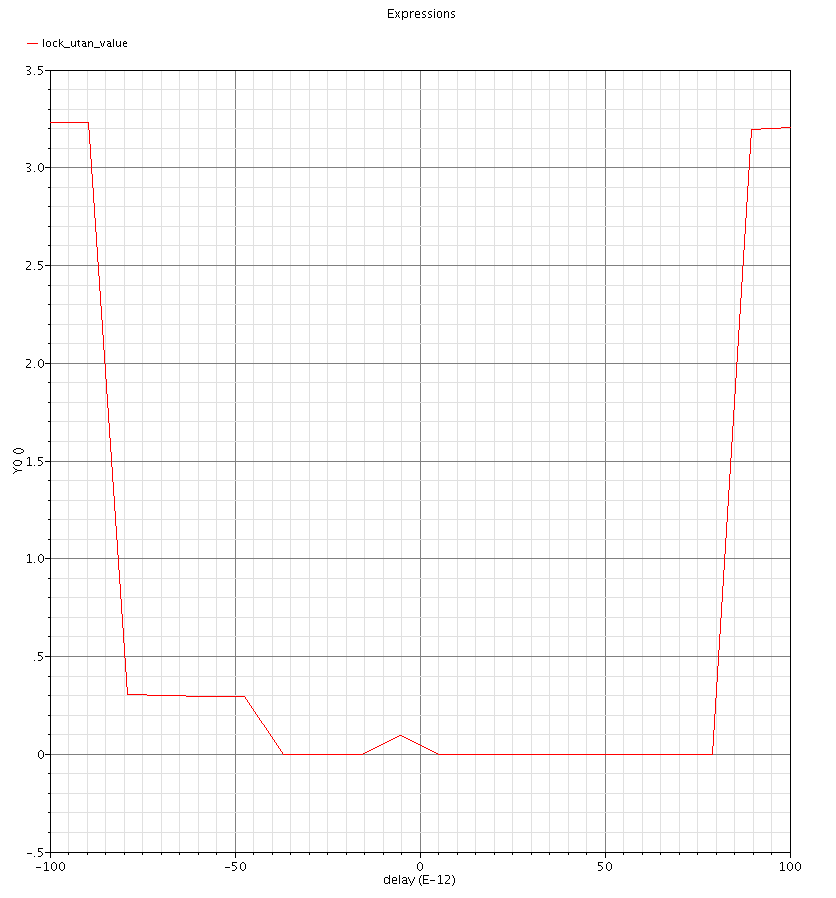
\includegraphics[width=0.65\textwidth]{../Bilder/LD_tran/LD_lsim_tm.png}
  \caption{Lock interval in typical mean}
  \label{fig:LDtm}
\end{figure}

\clearpage


\subsection{Frequency Multiplier}
To reach the wanted functionality the supply voltage and input frequency must be
adjusted in some of the corner variations. But with some tweaking a
multiplication of four can be reached in all the corners.

\section{Evaluation Plan and PAD List}
% Hur ska chippet testas?
% Vilken sorts PAD vart?
% Meningen med alla pinnar
% Sketch hur kontakterna ska kopplas till omvärlden

\section{Risks}
% Vad kan gå fel
\subsection{Phase Detector}
One of the biggest risks concerning the PD is when we get
slow/slow transistors, since the PD is used both as a stand-alone
module, and within the lock detector.
\subsection{Counter}
As the Counter is used to control the delay line, the speed and timing is not as big an issue as in the case of the other parts. The only issue that has occurred is that of the timing of the carry propagation signal and the inputs. When the transistor level Counter was tested, the input signals did not have to be clocked. In the layout this resulted in glitches where the upper bits acted as if the counter was counting up while the lower bits counted down as the input signals indicated. This problem occurred when the input signals switched too close in time to the switching of the clock. In this design the problem is solved by sampling the input signals through DFFs, but it can be easily overlooked as the signals appear to be sampled by the same clock if the parasitic capacitances of the wires, and the delays induced by these, are overlooked.
The carry propagation is the critical path of the Counter and therefore determines the maximum frequency at which it can operate. As this design has a 6-bit Counter the carry propagation path is quite long. Thus it is important to size the transistors for maximum speed.
\subsection{Digitally Controlled Delay Line}
\subsection{Lock Detector}
The main risk with the lock detector is if the lock signal goes low on a bad interval such that it causes the DLL output faulty signal.

% Bild på hur bra VS dåligt interval är

Related to this is also if it does not lock at all and thus is just a load on the chip. 
\subsection{Frequency Multiplier}

\section{Evaluation}
% Vad har vi lärt oss
% Hur har gruppen fungerat
% Har tiden delats väl
% Vad var bra/dåligt
% Vad bör ändras
% Kommentarer till kursen

\newpage
\appendix 
\newpage

\addcontentsline{toc}{section}{References}
\begin{thebibliography}{99}
        \bibitem{dll_clock}\textit{A Low-Power Digital DLL-Based Clock Generator in Open-Loop Mode - }
                Behzad Mesgarzadeh, Atila Alvandpour \\
                IEEE Journal of Solid-State Circuits. Vol. 44. No. 7. July 2009
        \bibitem{lock_detect}\textit{A 62.5-625-Mhz Anti-Reset All-Digital Delay-Locked Loop - }
                Shao-Ku Kao, Bo-Jiun Chen and Shen-Iuan Liu \\
                IEEE Transations on Circuits and Systems - II: Express Briefs, Vol. 54 No. 7, July 2007
        \bibitem{dll_report}\textit{DLL-Based Frequency Multiplier - }
                Layout Edition 2008-05-25 \\
        \bibitem{transistor}\textit{Transistor Level - }
                Bengtz, Berneland, Björklund, Hallberg, Svensk \\

\end{thebibliography}

\newpage
\section{Corner simulation results}
\label{sec:corners}

\begin{figure}[h]
  \centering
  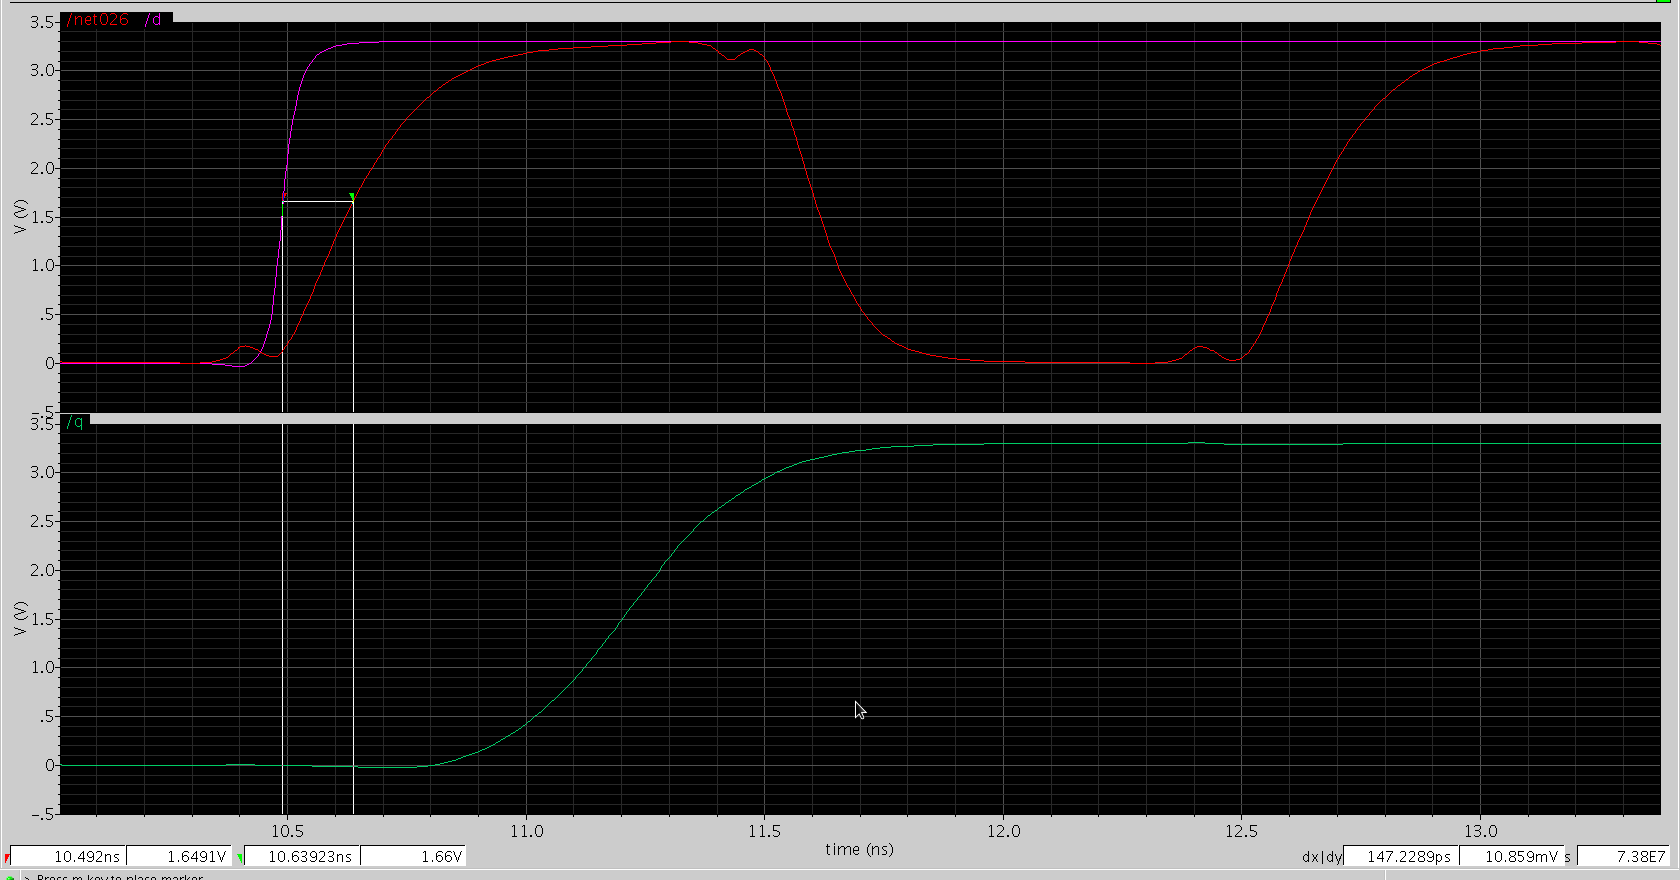
\includegraphics[width=0.65\textwidth]{../Bilder/Layout/simulations/pd_tm.png}
  \caption{Set-up time of PD in typical mean}
  \label{fig:PDtm}
\end{figure}

\begin{figure}[h]
  \centering
  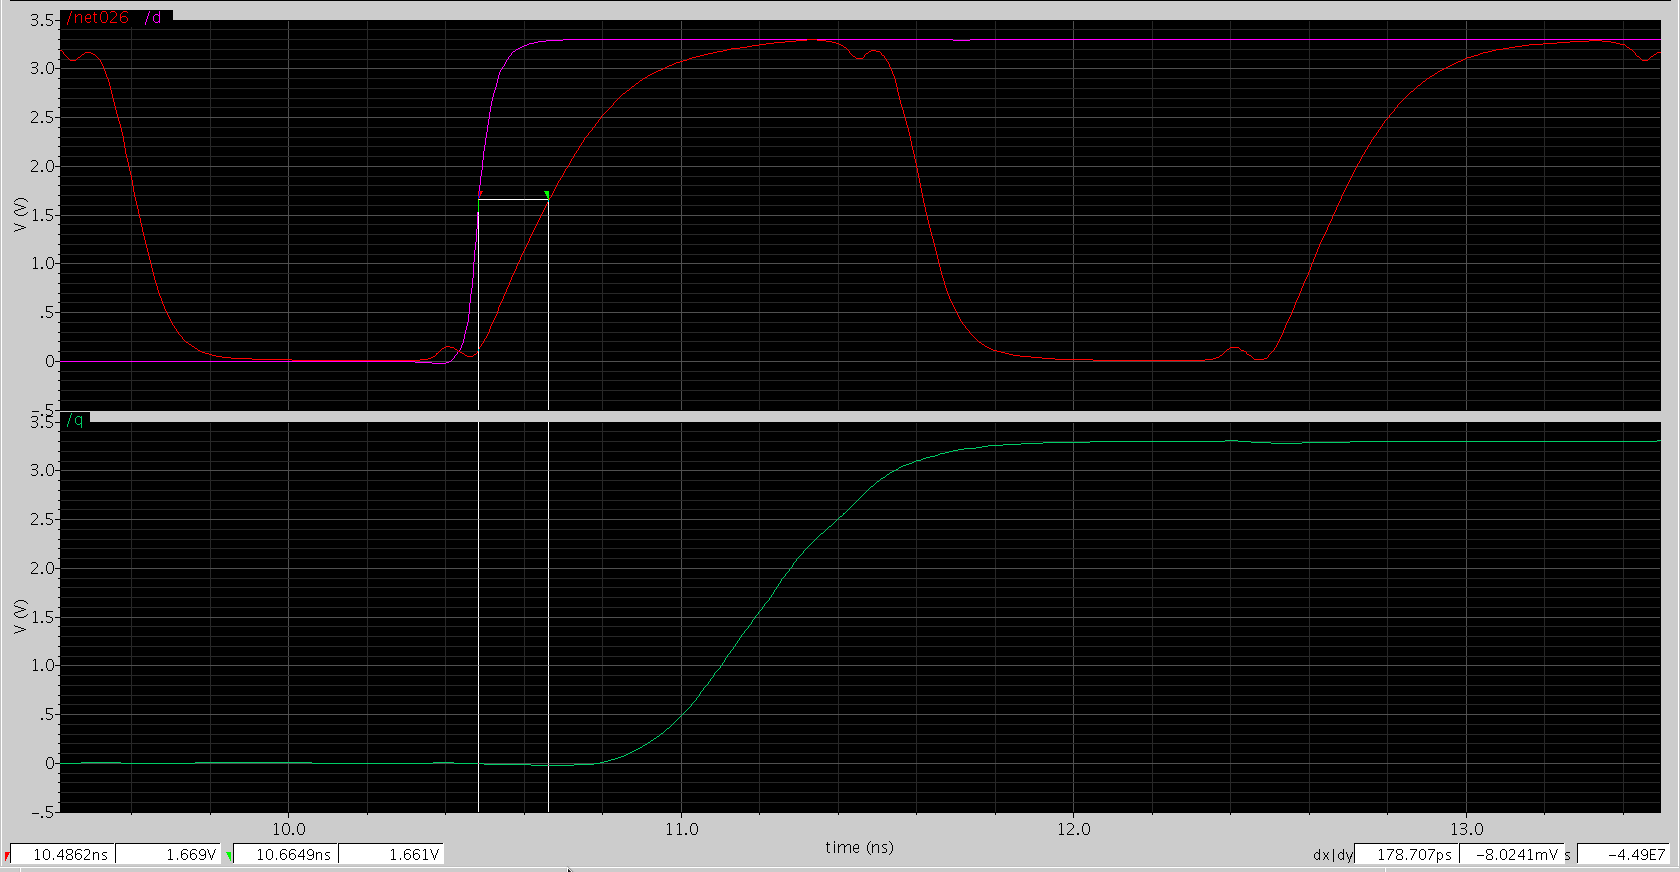
\includegraphics[width=0.65\textwidth]{../Bilder/Layout/simulations/pd_wo.png}
  \caption{Set-up time of PD in worst one}
  \label{fig:PDwo}
\end{figure}

\begin{figure}[h]
  \centering
  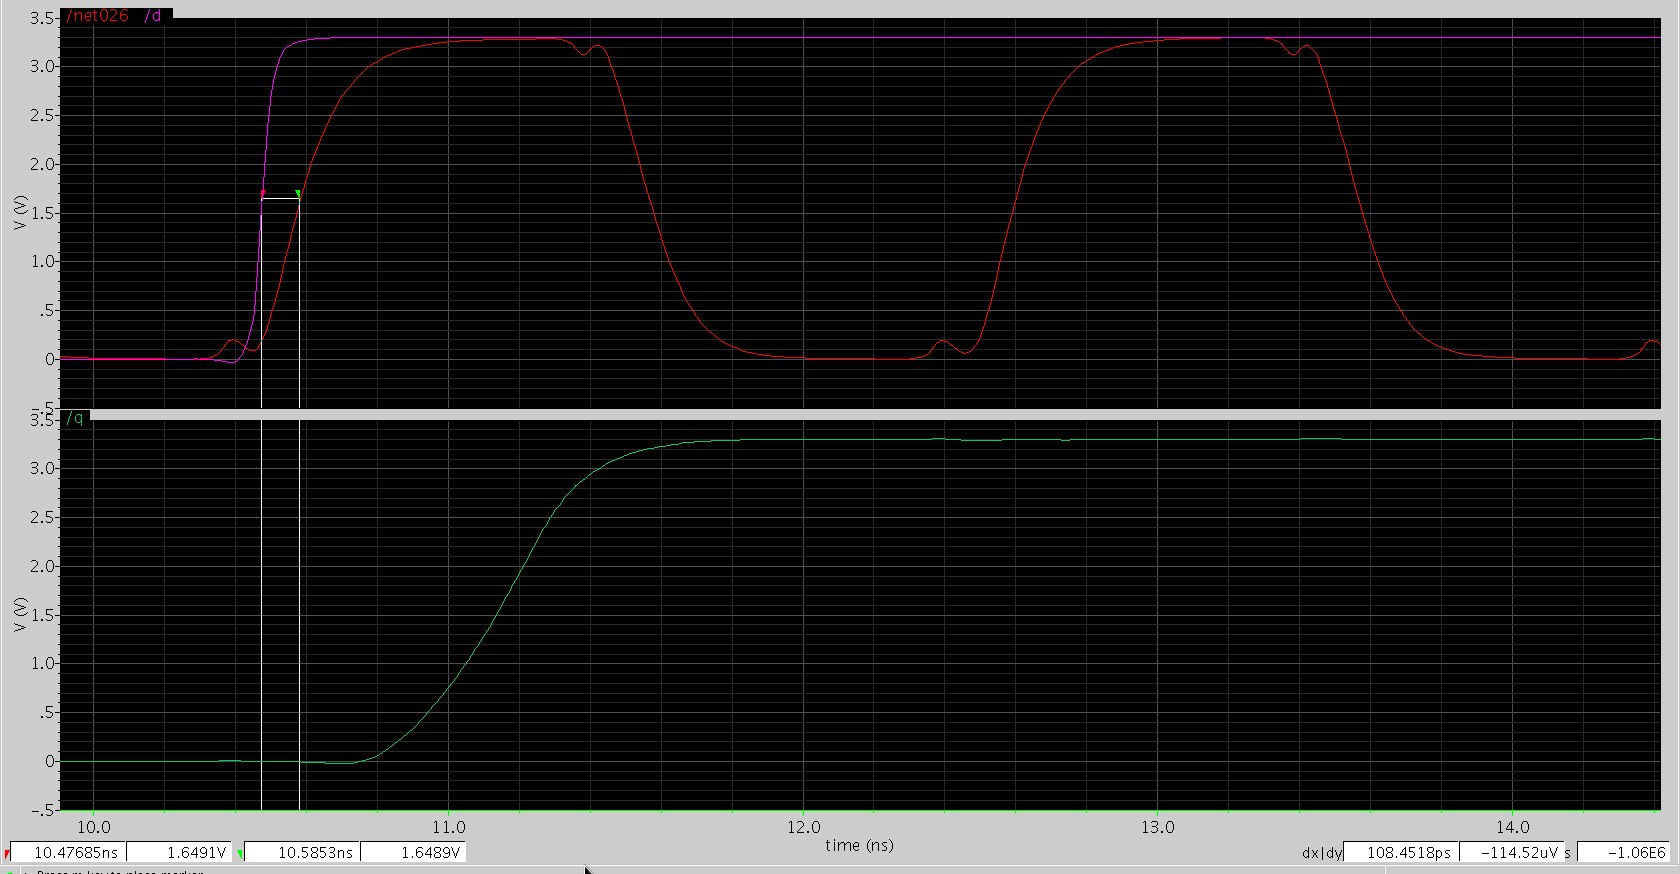
\includegraphics[width=0.65\textwidth]{../Bilder/Layout/simulations/pd_wz.png}
  \caption{Set-up time of PD in worst zero}
  \label{fig:PDwz}
\end{figure}

\begin{figure}[h]
  \centering
  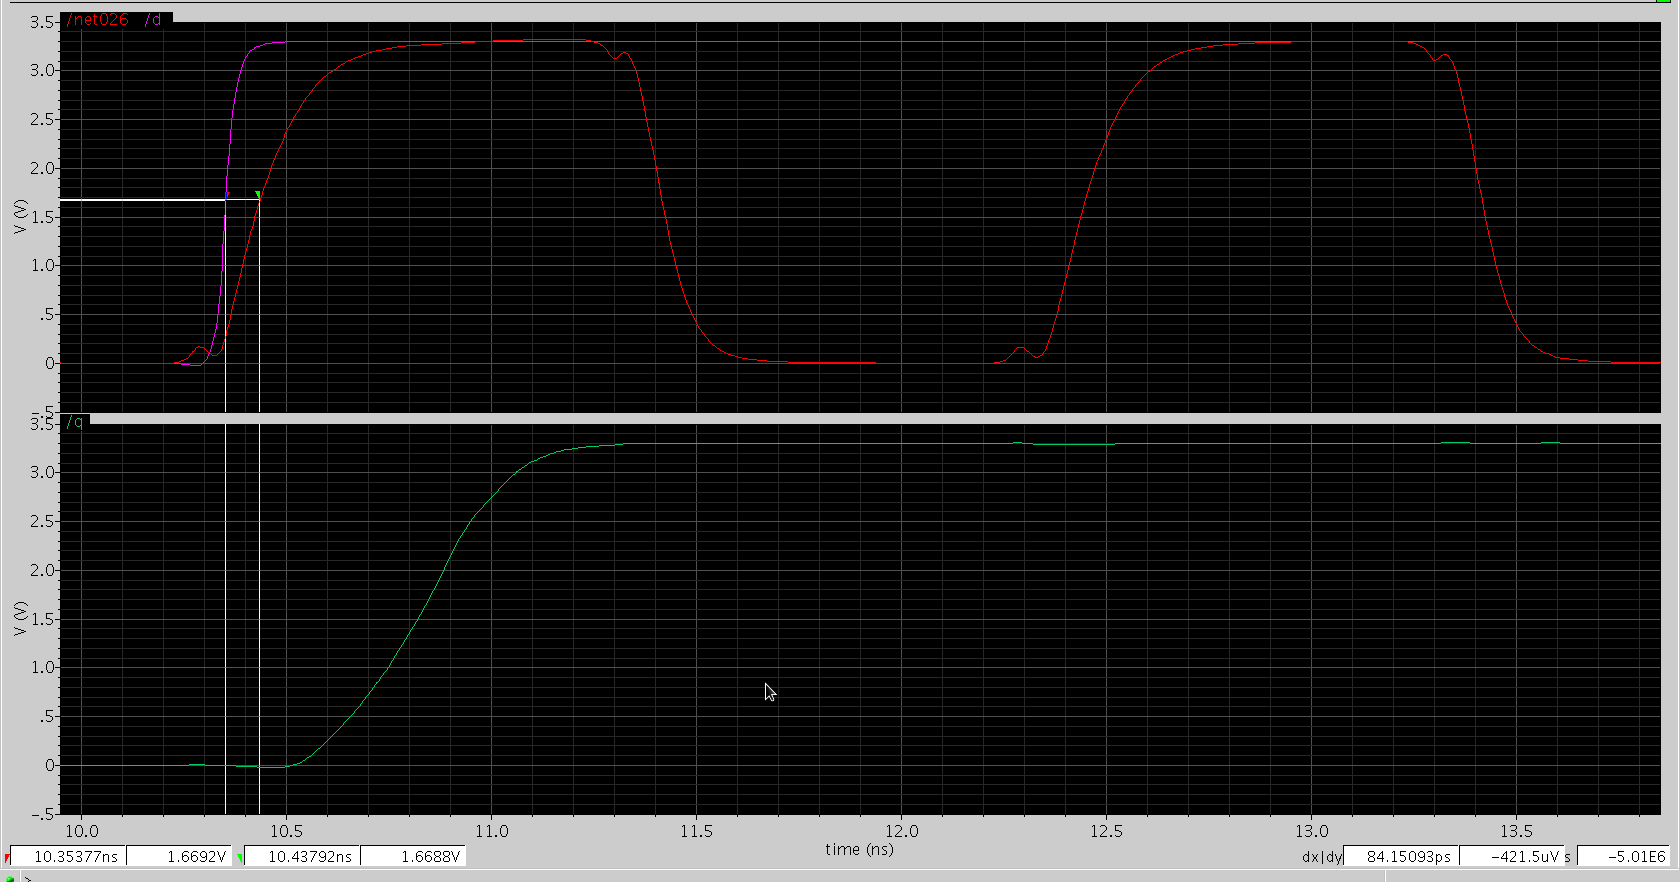
\includegraphics[width=0.65\textwidth]{../Bilder/Layout/simulations/pd_wp.png}
  \caption{Set-up time of PD in worst power}
  \label{fig:PDwp}
\end{figure}

\begin{figure}[h]
  \centering
  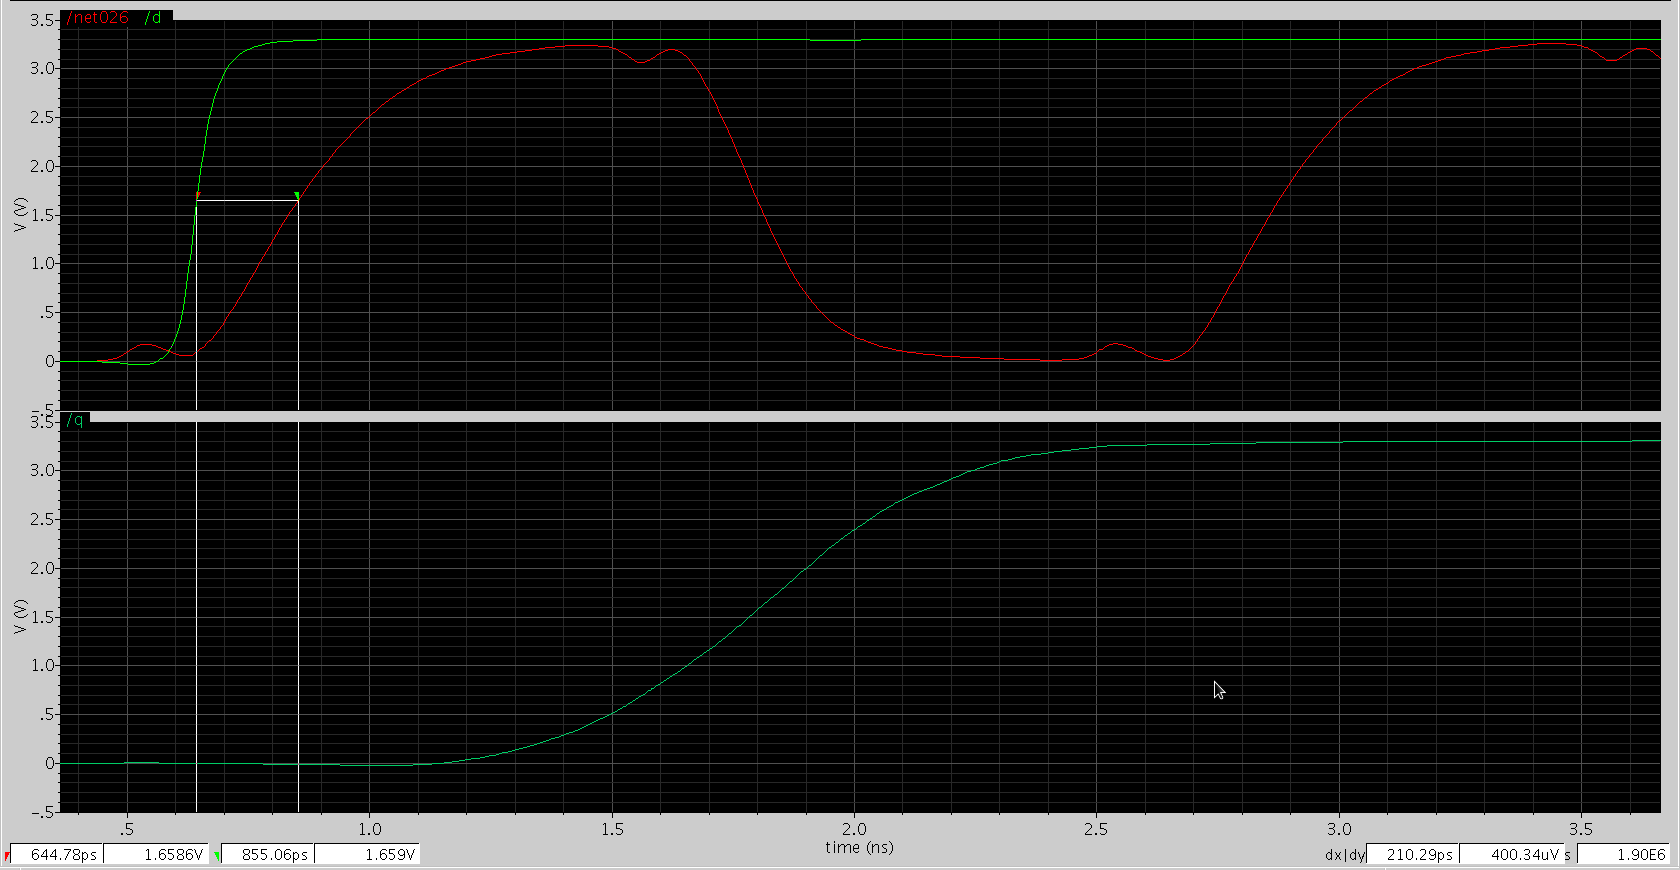
\includegraphics[width=0.65\textwidth]{../Bilder/Layout/simulations/pd_ws.png}
  \caption{Set-up time of PD in worst slow}
  \label{fig:PDws}
\end{figure}


In figure \ref{fig:LDwp} to \ref{fig:LDws} the corner simulations for
the lock interval is shown.

\begin{figure}[h]
  \centering
  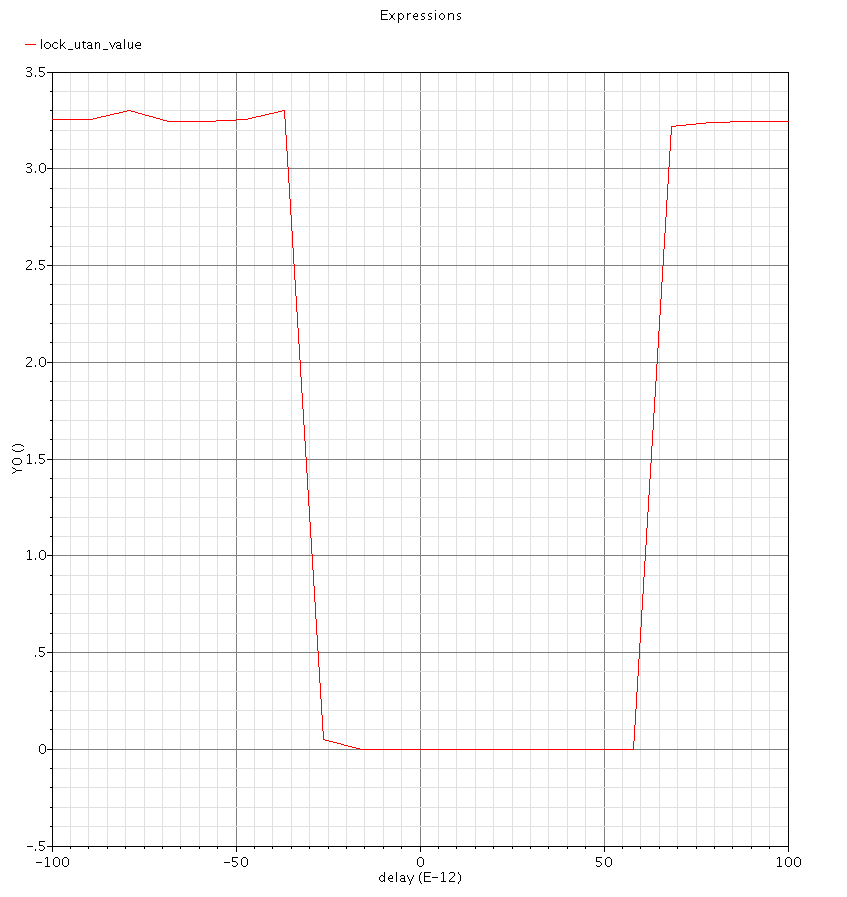
\includegraphics[width=0.65\textwidth]{../Bilder/LD_tran/LD_lsim_wp.png}
  \caption{Lock interval in worst power}
  \label{fig:LDwp}
\end{figure}

\begin{figure}[h]
  \centering
  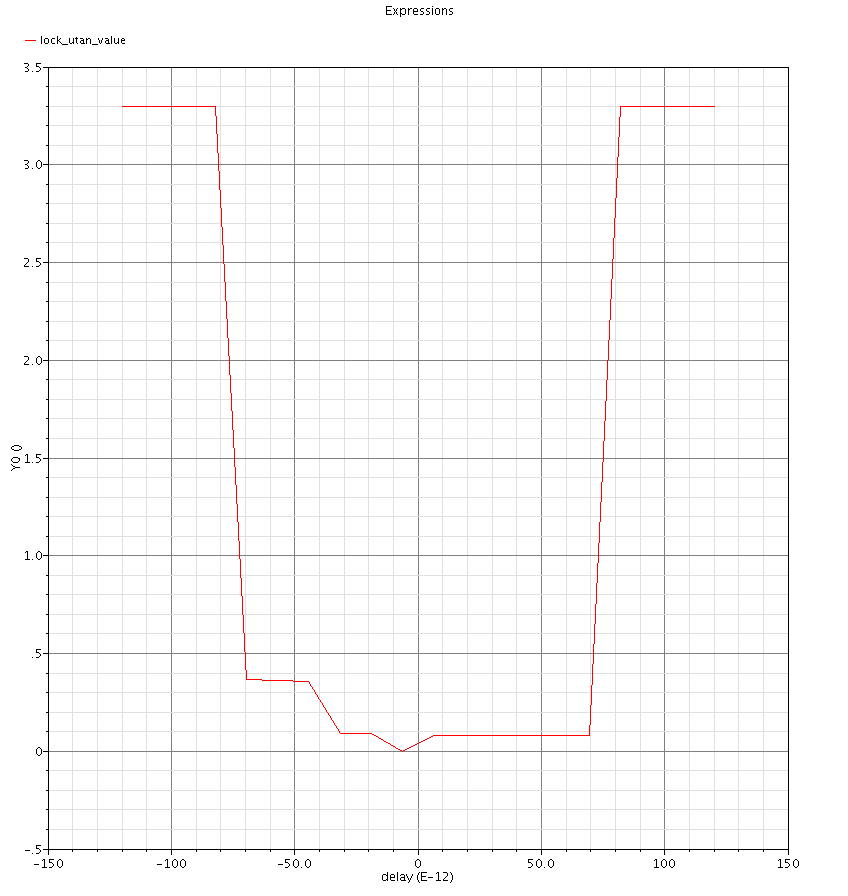
\includegraphics[width=0.65\textwidth]{../Bilder/LD_tran/LD_lsim_wo.png}
  \caption{Lock interval in worst one}
  \label{fig:LDwo}
\end{figure}

\begin{figure}[h]
  \centering
  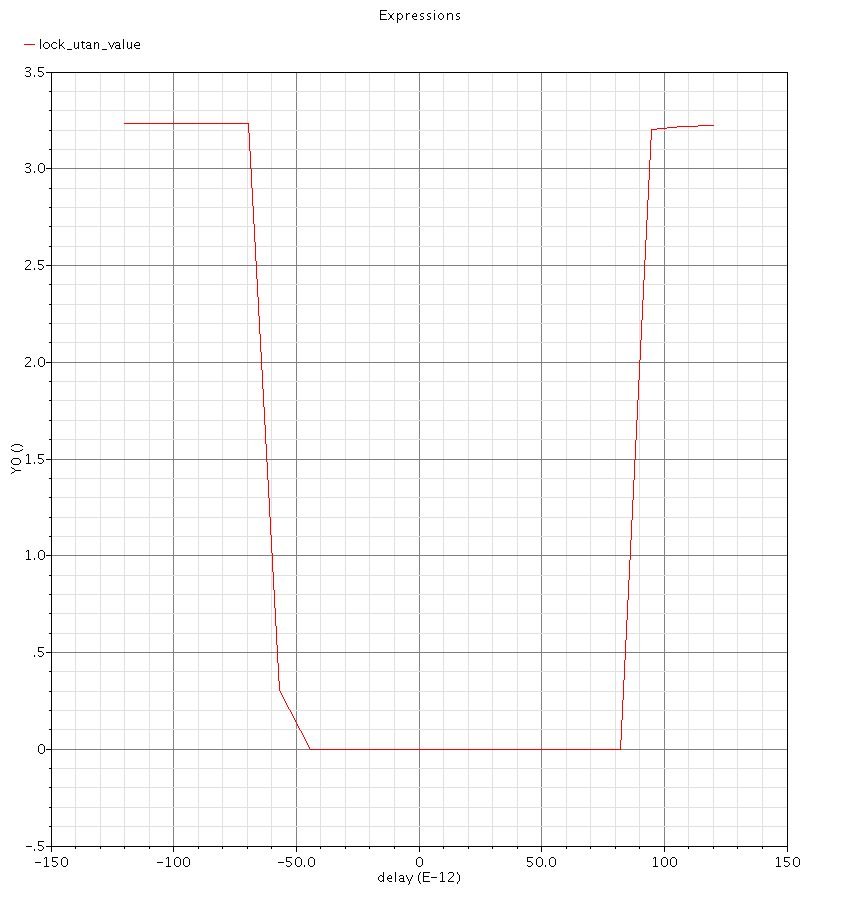
\includegraphics[width=0.65\textwidth]{../Bilder/LD_tran/LD_lsim_wz.png}
  \caption{Lock interval in worst zero}
  \label{fig:LDwz}
\end{figure}

\begin{figure}[h]
  \centering
  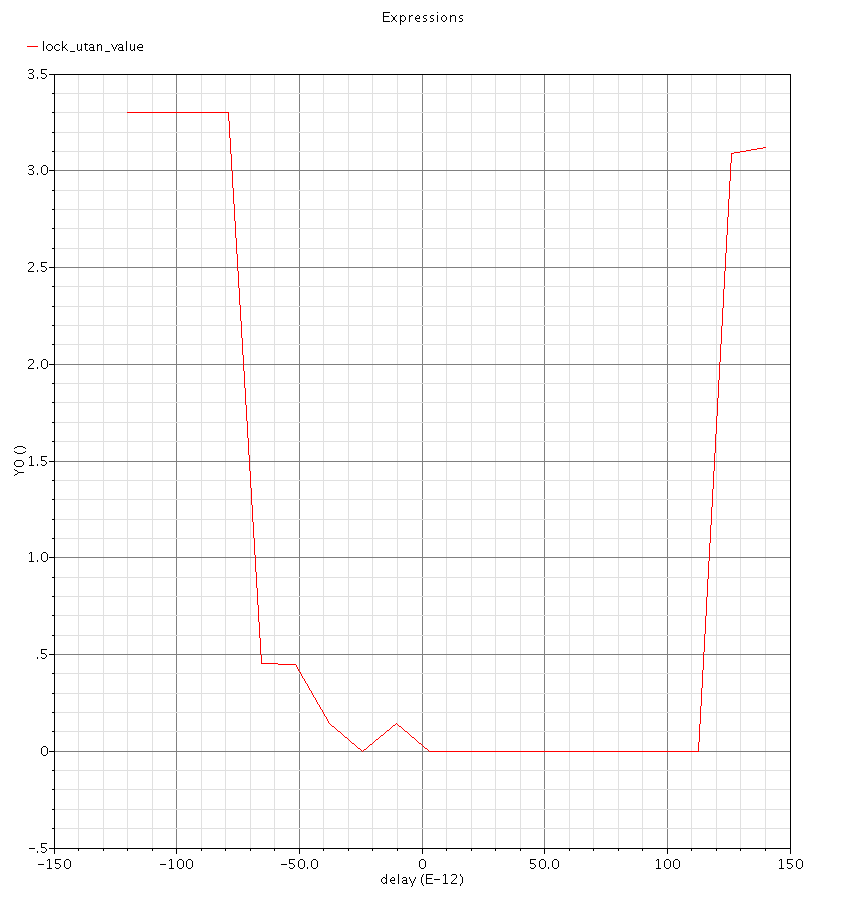
\includegraphics[width=0.65\textwidth]{../Bilder/LD_tran/LD_lsim_ws.png}
  \caption{Lock interval in worst slow}
  \label{fig:LDws}
\end{figure}

\section{Layout of sub-blocks}
\label{sec:Layout}

\begin{figure}[h]
  \centering
  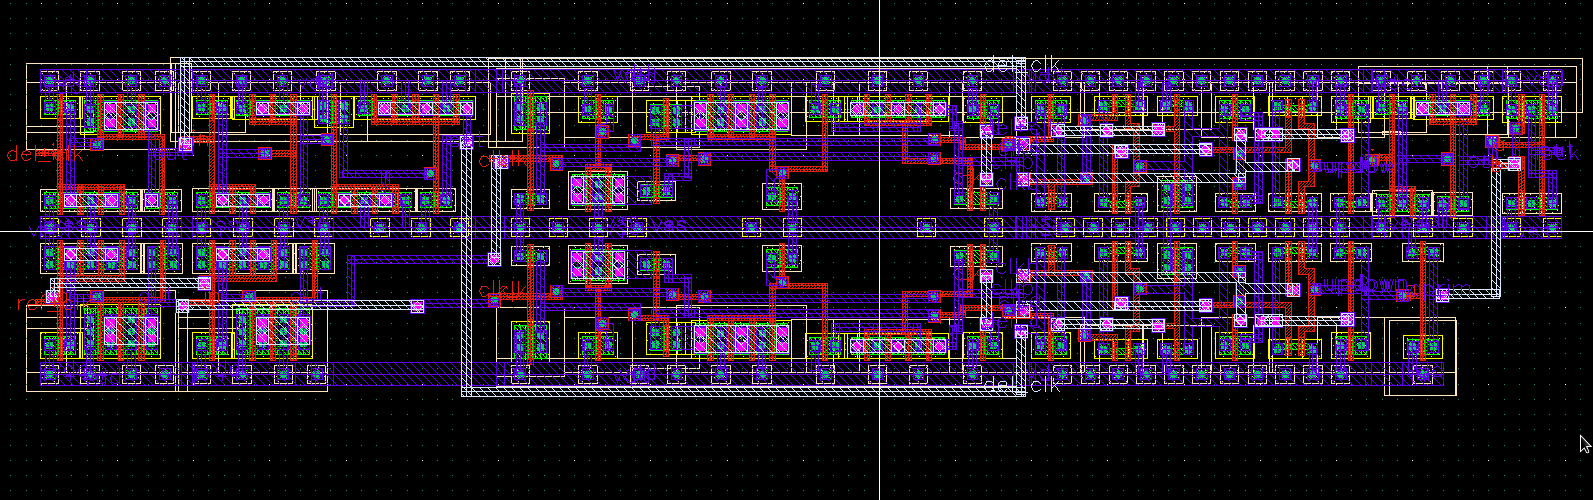
\includegraphics[width=1.0\textwidth]{../Bilder/Layout/lock_detector.png}
  \caption{Lock Detector layout}
  \label{fig:LD}
\end{figure}

\begin{figure}[h]
  \centering
  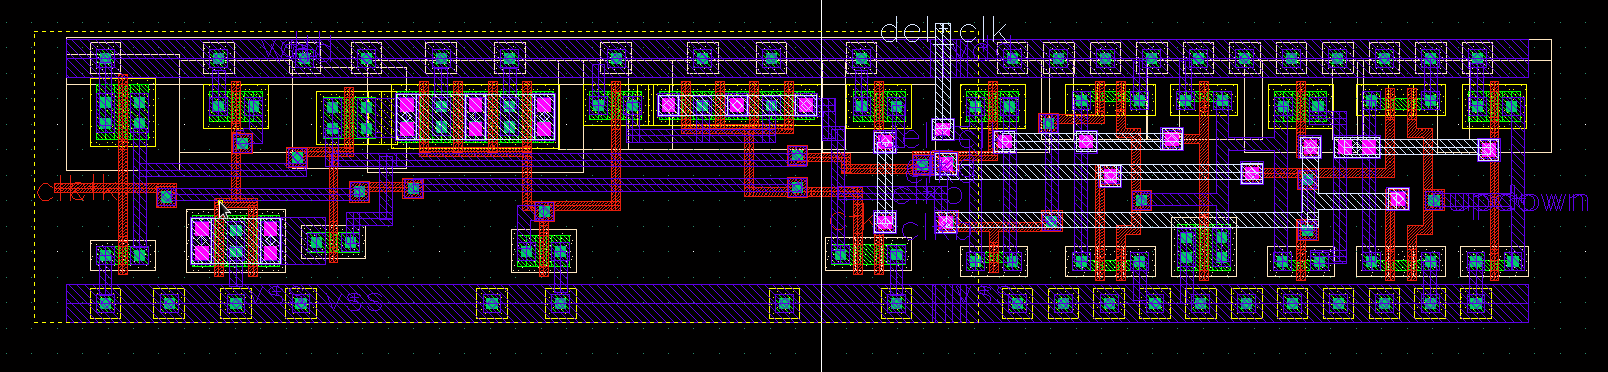
\includegraphics[width=1.0\textwidth]{../Bilder/Layout/pd_including_clk_set.png}
  \caption{PD layout}
  \label{fig:pd_final}
\end{figure}

\begin{figure}[h]
  \centering
  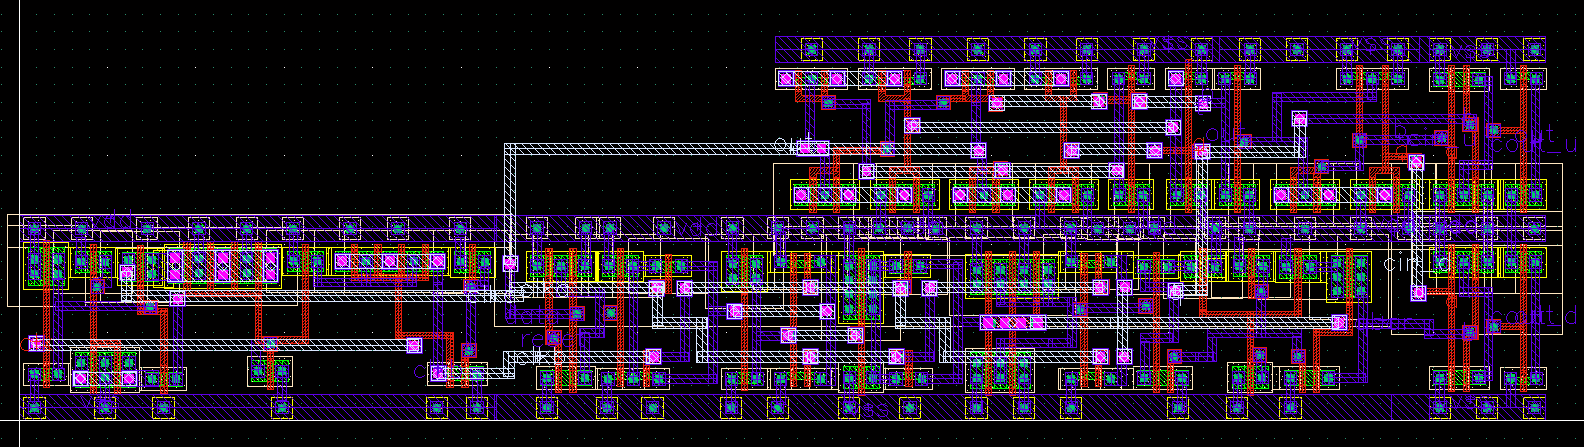
\includegraphics[width=1.0\textwidth]{../Bilder/Layout/bitcell.png}
  \caption{Lock Detector layout}
  \label{fig:bitcell_final}
\end{figure}

\begin{figure}[h]
  \centering
  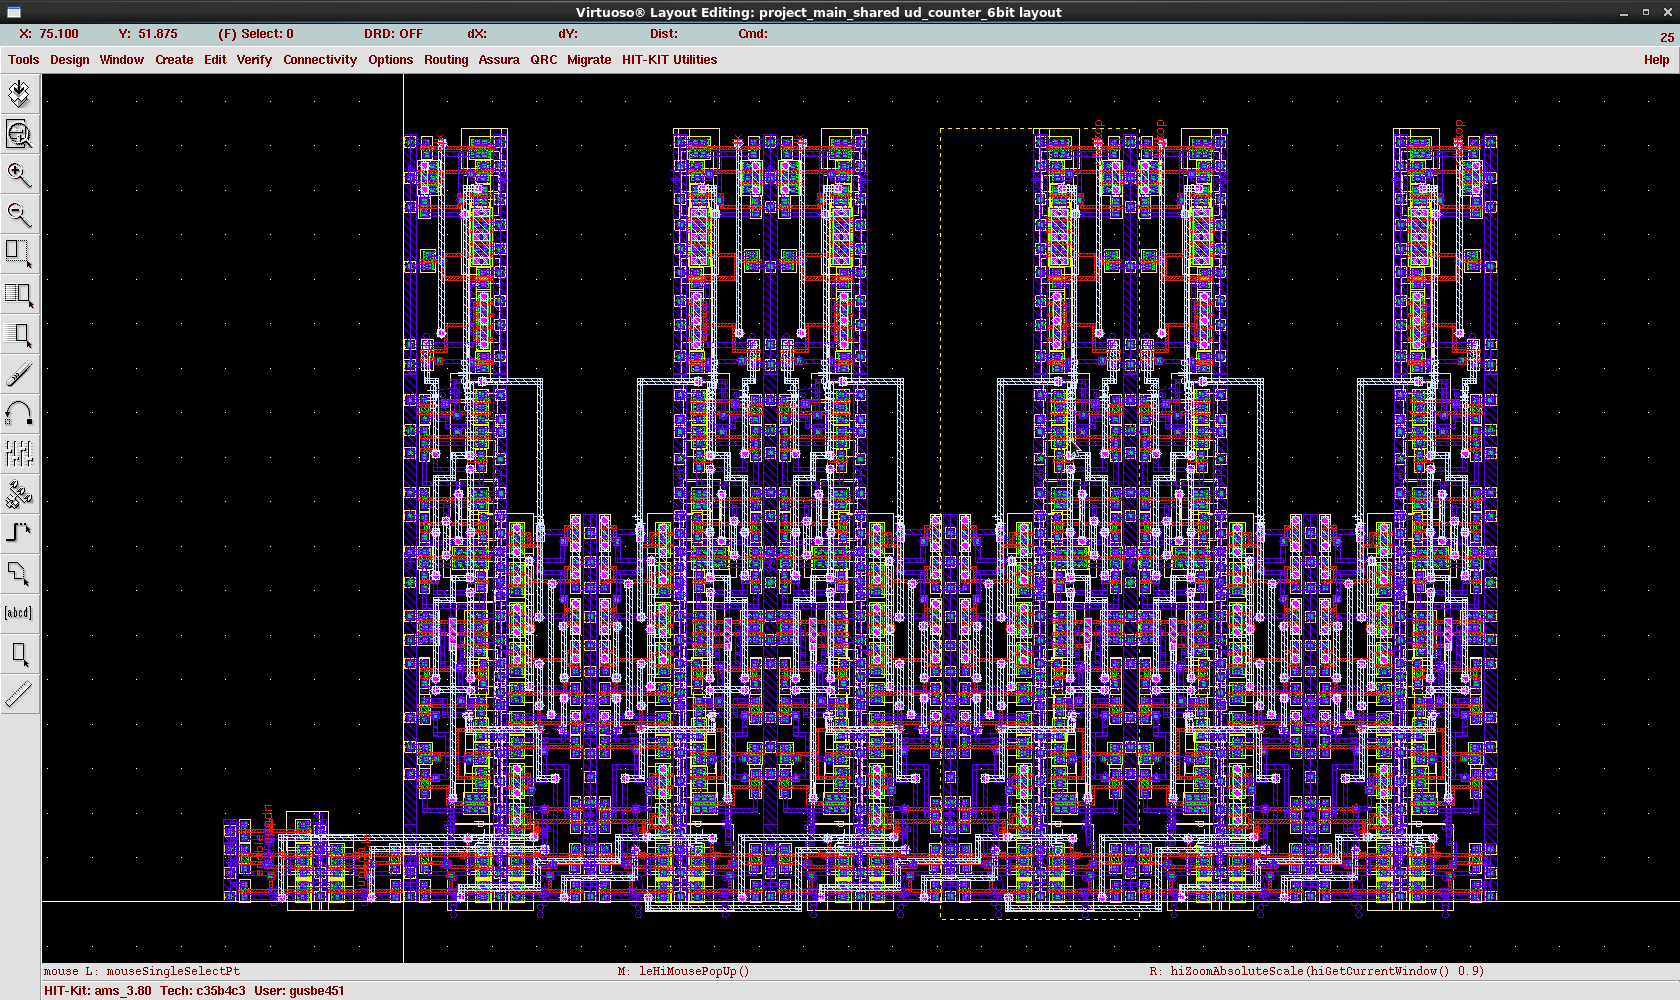
\includegraphics[width=1.0\textwidth]{../Bilder/Layout/ud_counter_6bit.png}
  \caption{UD counter layout}
  \label{fig:counter_final}
\end{figure}

\begin{figure}[h]
  \centering
  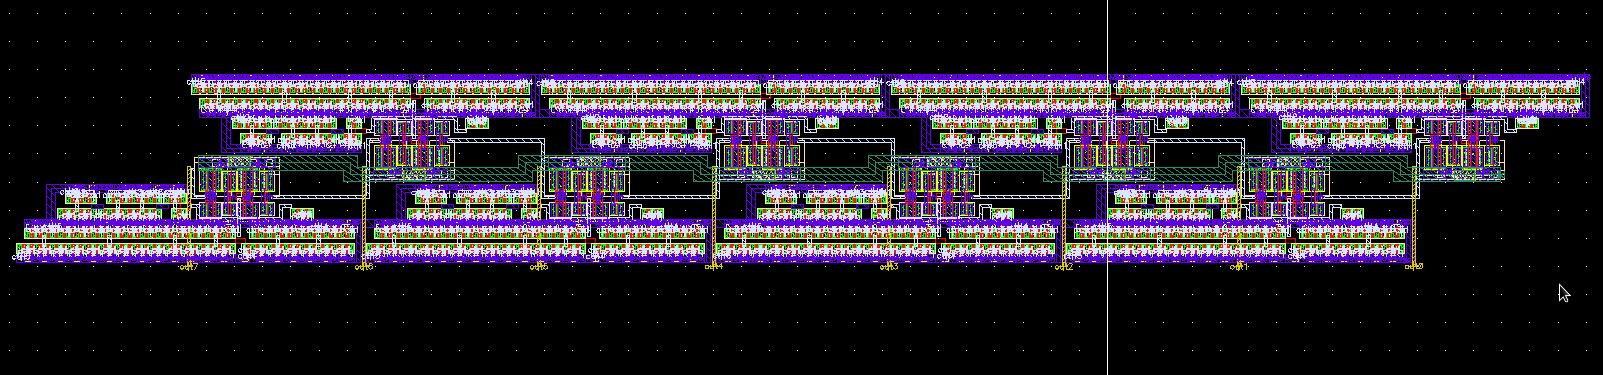
\includegraphics[width=1.0\textwidth]{../Bilder/Layout/delay_line_trans.png}
  \caption{Delay line layout}
  \label{fig:delay_final}
\end{figure}

\begin{figure}[h]
  \centering
  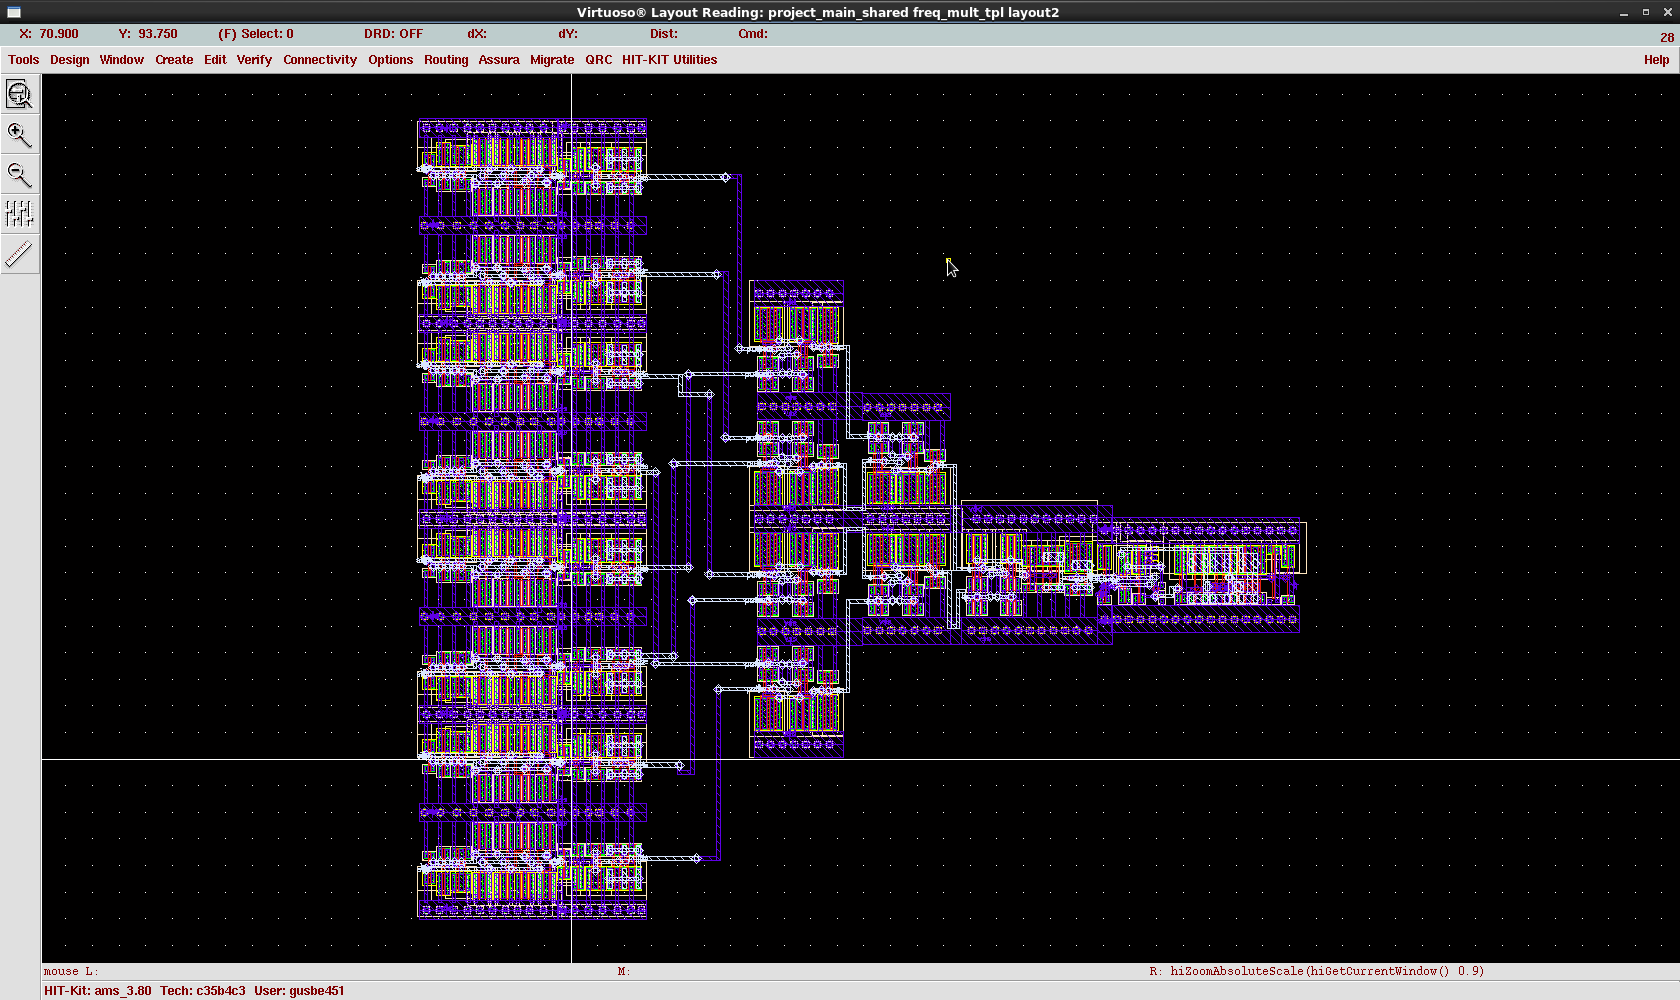
\includegraphics[width=1.0\textwidth]{../Bilder/Layout/freq_mult_tpl.png}
  \caption{Freqmult layout}
  \label{fig:freq_mult_final}
\end{figure}

\begin{figure}[h]
  \centering
  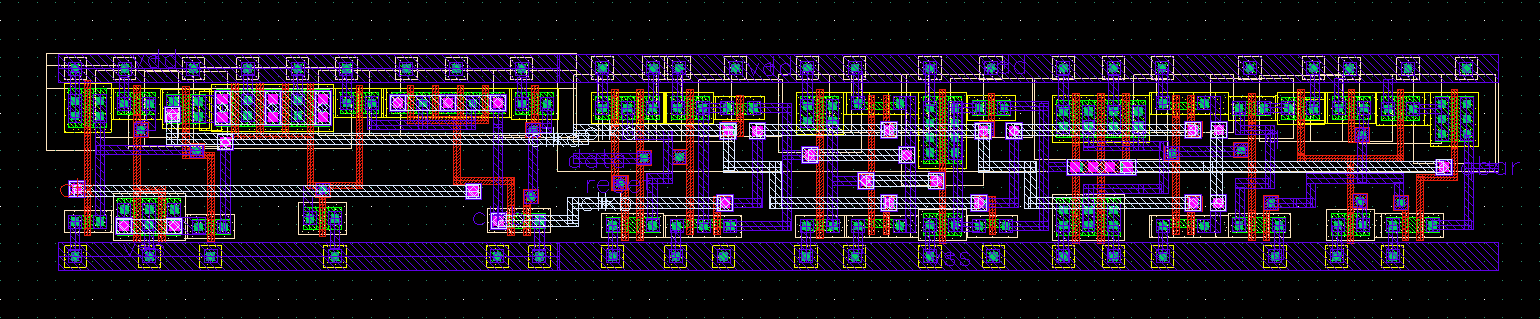
\includegraphics[width=1.0\textwidth]{../Bilder/Layout/dff_sync_reset_qbar_clkset.png}
  \caption{DFF layout}
  \label{fig:dff_final}
\end{figure}

\begin{figure}[h]
  \centering
  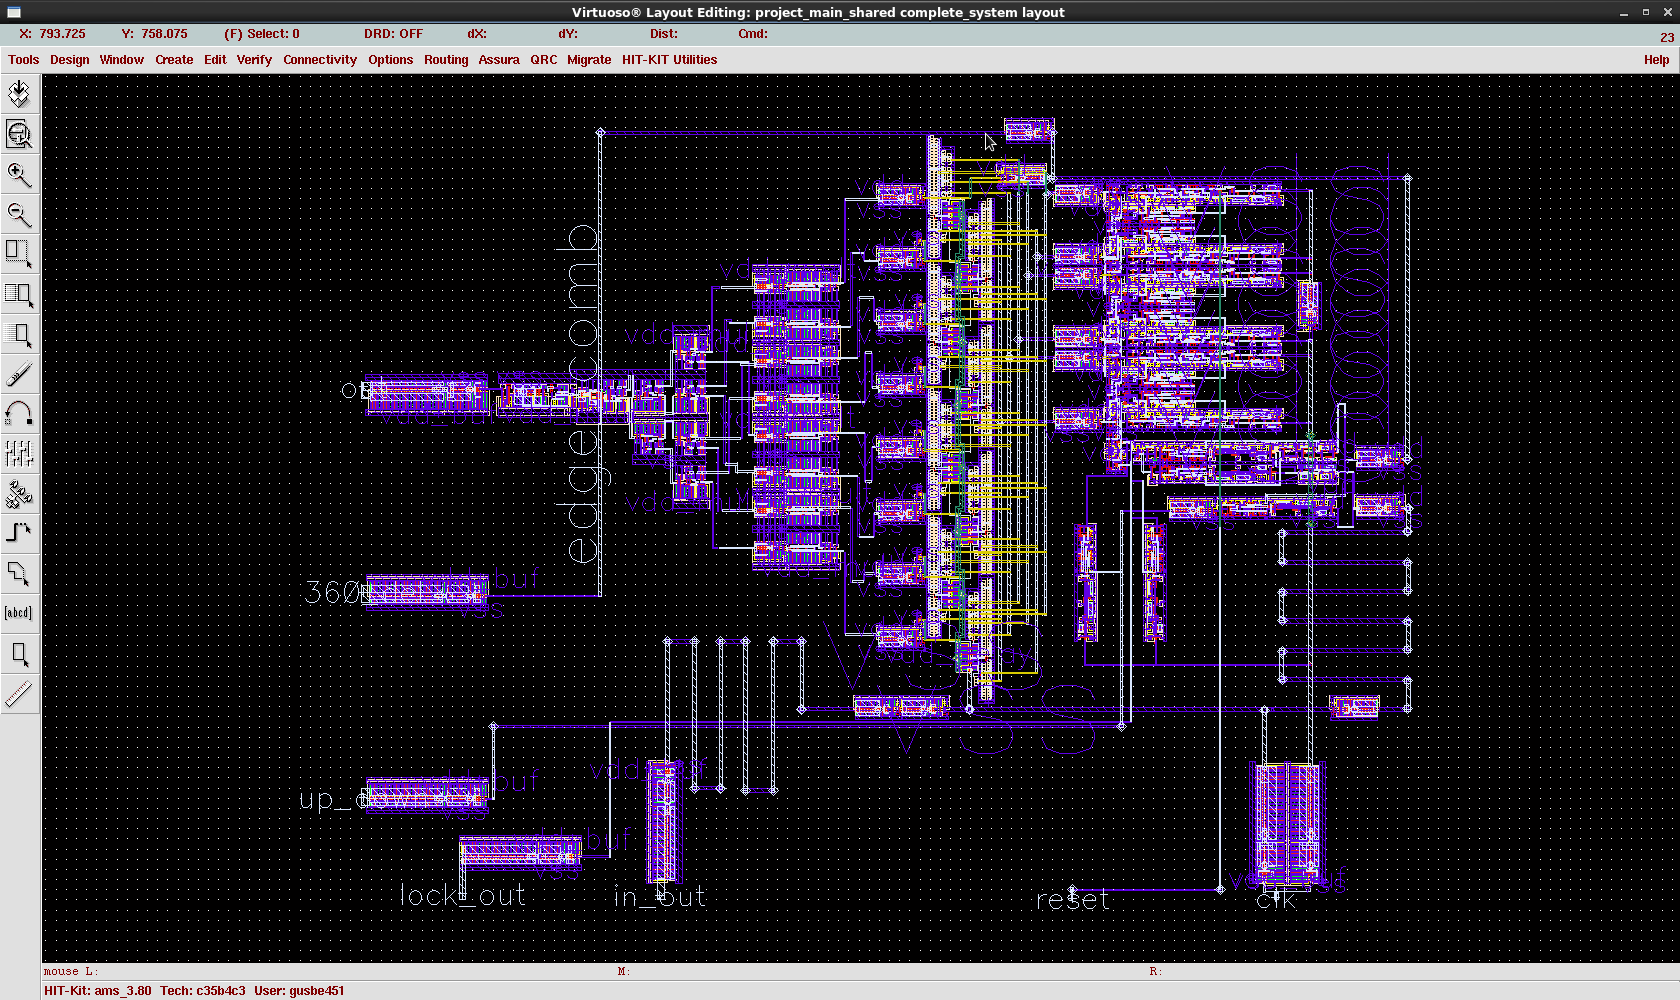
\includegraphics[width=1.0\textwidth]{../Bilder/Layout/complete_system.png}
  \caption{Complete system layout}
  \label{fig:complete_system_final}
\end{figure}

\end{document} 
% Local Variables: %%% mode: latex %%% TeX-master: t %%% End:
